% CycloBench paper skeleton (workshop version, 8 pages + references)
% Compile: tectonic main.tex
\documentclass[10pt]{article}
\usepackage[margin=1in]{geometry}
\usepackage{times}
\usepackage{booktabs}
\usepackage{graphicx}
\usepackage{amsmath,amssymb}
\usepackage{hyperref}
\usepackage{natbib}
\usepackage{xcolor}
\usepackage{enumitem}
\usepackage{caption}
\usepackage{indentfirst}
\captionsetup{font=small,labelfont=bf}

\newcommand{\todo}[1]{\textcolor{red}{[TODO: #1]}}
\newcommand{\method}{CycloBench}

\title{\method: A Verifiable Benchmark for LLM Reasoning on Cyclostratigraphic Data}
\author{Kehan Yu\thanks{Peking University. Correspondence: phenomenologicallife.}}
\date{}

\begin{document}
\maketitle

\begin{abstract}
Large language models are increasingly used as scientific assistants, yet their ability to
perform quantitative geoscientific analysis remains poorly measured. We introduce \method, a
verifiable benchmark for cyclostratigraphic analysis of sedimentary sequences. \method\ pairs
synthetic dual-well records with exact ground truth across six question families: sedimentation
(duration and mean rate), age models, hiatus detection, orbital attribution of spectral peaks,
amplitude modulation, and cross-well correlation. The benchmark contains \textbf{480 scored
items} from 60 instances (40 train / 20 test). Every item is scored 0/1 automatically, with two
rules that block known shortcuts (the modern 41-kyr obliquity and single-proxy peak
attribution). We release the generator, the instances, the scoring code and a fixed protocol
with three conditions -- zero-shot, chain-of-thought, and tool-augmented -- designed to
separate domain knowledge from tool use. Because the answers are verifiable, the benchmark also
serves as a reward environment for post-training; we outline a GRPO recipe for a 1.5B model and
release the code as a starting point for that use. In a first evaluation, five open models score
between 0.0\% and 15.6\% macro accuracy, and neither chain-of-thought prompting nor a
restricted Python sandbox closes the gap, so the benchmark remains far from saturation.
Code and data are at
\url{https://github.com/KhanKehan/CycloBench}.
\end{abstract}

\section{Introduction}
\label{sec:intro}
% 1 page
Large language models are increasingly used as scientific assistants, yet their ability to
perform quantitative geoscientific analysis remains poorly measured. Existing benchmarks focus
on textual knowledge or chart reading, not on the multi-step numerical workflow of
cyclostratigraphy: spectral estimation with red-noise testing, sedimentation-rate modelling,
astronomical tuning, and hiatus detection.

We argue that cyclostratigraphy is a useful testbed for \emph{verifiable} scientific reasoning:
data can be generated with known ground truth, answers are numeric or discrete, and correct
solutions require both domain knowledge and tool use. This matters for evaluation because
text-only benchmarks cannot distinguish a model that recites Milankovitch theory from one that
can estimate a sedimentation rate from a log; it matters for post-training because a verifiable
reward makes reinforcement learning possible without human preference labels, yet the reward
must survive a multi-step analysis rather than a single answer string.

Our contributions are:
\begin{itemize}[leftmargin=1.2em,itemsep=2pt]
  \item \method, a verifiable benchmark of 480 scored items across six task families, with exact
        ground truth, 0/1 scoring, and anti-cheat rules (\S\ref{sec:bench}).
  \item A fixed evaluation protocol with three prompting conditions and an error taxonomy
        that separates knowledge errors from tool-use and numerical errors
        (\S\ref{sec:setup}, \S\ref{sec:results}).
  \item A verifiable-reward recipe for post-training, released as code, with the zero-shot
        evaluation as the baseline it must beat (\S\ref{sec:grpo}).
\end{itemize}

\section{Related Work}
\label{sec:related}
% 0.75 page
\textbf{Benchmarks for language models.} HELM \citep{liang2022helm} and BIG-bench
\citep{srivastava2022bigbench} organise broad capability evaluations, while MMLU
\citep{hendrycks2021mmlu} and GPQA \citep{rein2023gpqa} test knowledge through multiple-choice
questions. SciBench \citep{wang2023scibench} moves to college-level problem solving but still
scores a short final answer. None of these require the model to analyse raw measurements and
return numbers that follow from the data, which is the setting of \method. Agentic benchmarks
such as ScienceAgentBench \citep{chen2024scienceagentbench}, MLE-bench \citep{chan2024mlebench},
SciCode \citep{tian2024scicode} and LAB-Bench \citep{laurent2024labbench} evaluate end-to-end
task completion or research coding; \method\ instead isolates a single numerical workflow with
exact, per-question ground truth.

\textbf{Tool use and scientific workflows.} ReAct \citep{yao2023react} interleaves reasoning
and actions, and Toolformer \citep{schick2023toolformer} teaches models to call APIs. Our
tool-augmented condition follows this line, but the tool here is a numerical analysis stack
over a data file, and the evaluation checks the final numbers rather than the trajectory.
MassSpecGym \citep{bushuiev2024massspecgym} is the closest benchmark in the adjacent
mass-spectrometry domain and also centres on ranked structure candidates.

\textbf{Cyclostratigraphy.} Astronomical tuning relates sedimentary cycles to orbital forcing
\citep{hinnov2007ats, hinnov2013cyclo}. The 405-kyr eccentricity cycle provides a metronome,
while obliquity and precession periods differ at 300 Ma from their modern values; hiatuses
break phase continuity and must be detected before tuning. The standard toolchains,
astrochron \citep{meyers2014astrochron} and Acycle \citep{li2019acycle}, implement these steps.

\textbf{Post-training with verifiable rewards.} GRPO \citep{shao2024deepseekmath} replaces the
value network of PPO with group-normalised advantages and has become a standard recipe for
reinforcement learning with verifiable rewards (RLVR) on math \citep{yang2024qwenmath}. Process
supervision \citep{lightman2023verify} and large post-training pipelines \citep{lambert2024tulu3}
study how far such signals scale, while preference optimisation \citep{rafailov2023dpo} and RLHF
\citep{ouyang2022instructgpt} address alignment rather than correctness. Whether RLVR transfers
to scientific data analysis, where the reward requires running an analysis rather than matching
a final answer string, is largely untested.

\section{\method}
\label{sec:bench}
% 1.5 pages
\subsection{Task suite}
\method\ contains six task families (Table~\ref{tab:tasks}). Each item provides two wells of
synthetic log data and asks for numeric or discrete answers that are checked exactly.

\begin{table}[t]
\centering
\small
\begin{tabular}{@{}llll@{}}
\toprule
Family & Questions & Answer type & Tolerance \\
\midrule
Sedimentation & Q1 duration, Q4 mean SR & float (Myr, cm/kyr) & 0.10 / 0.20 \\
Age model & Q2 age at 250 m & float (Ma) & 0.050 \\
Hiatus & Q3 depths and durations & list of (m, kyr) & 3 m / 50 kyr \\
Orbital attribution & Q6 60/112-kyr peaks & 4 booleans & exact \\
Modulation & Q7 amplitude modulation & bool + 2 floats & exact / range \\
Cross-well & Q8 shared hiatus & 3 floats & 3 m / 50 kyr \\
\bottomrule
\end{tabular}
\caption{Question families in \method. Every instance asks all eight questions
(Q1--Q8); Q1/Q4 share the sedimentation family and Q3/Q8 share the hiatus family.}
\label{tab:tasks}
\end{table}

\subsection{Data generation}
Each instance is a forward simulation on a 1-kyr grid over $T \in [5.0, 7.8]$ Myr.
Sedimentation rate follows a smooth low-frequency profile with a step change, drawn
from 6.7--8.6 cm/kyr, and is set to zero during hiatus events (80--420 kyr each,
constrained to be non-overlapping). Depth is the integral of the rate, so a hiatus
produces a condensed interval in which age jumps while depth advances little.

Signals mix the 405-kyr and 100-kyr eccentricity terms, obliquity at the simulated
300-Ma period (32--36.5 kyr), and precession (18--21 kyr), with an AR(1) background.
GR additionally carries autogenic 60- and 112-kyr cycles; CARB does not, and its
obliquity amplitude is modulated at ~170 kyr more strongly than GR. Well B shares the
regional hiatus but has a different rate profile and its own local hiatuses, so the
same event appears at different depths in the two wells.

\begin{table}[t]
\centering
\small
\begin{tabular}{@{}lcccccc@{}}
\toprule
Split & Instances & Duration (Myr) & Depth A (m) & SR (cm/kyr) & Hiatuses & Obliquity (kyr) \\
\midrule
Train & 40 & 5.0--7.8 & 291--597 & 5.5--7.8 & 3--5 & 32.0--36.4 \\
Test & 20 & 5.2--7.7 & 299--558 & 5.6--8.1 & 3--5 & 32.4--36.5 \\
\bottomrule
\end{tabular}
\caption{Benchmark statistics. Each instance yields eight scored questions, so the
benchmark contains 480 items in total.}
\label{tab:stats}
\end{table}

\subsection{Scoring and anti-cheat}
Each question is scored 0/1 with the tolerances in Table~\ref{tab:tasks}. Two rules
target shortcuts: an answer of 41 kyr to Q5 is rejected because the obliquity period at
300 Ma differs from the modern value, and Q6 requires cross-validation between GR and
CARB, so reporting a peak in one proxy alone does not earn credit. The final score of an
instance is the fraction of its eight questions that pass. The generator writes the
latent parameters to disk, so every truth value is known exactly rather than estimated, and
generation is deterministic given the instance id (re-running the generator reproduces the
same truth file byte for byte).

\begin{figure}[t]
\centering
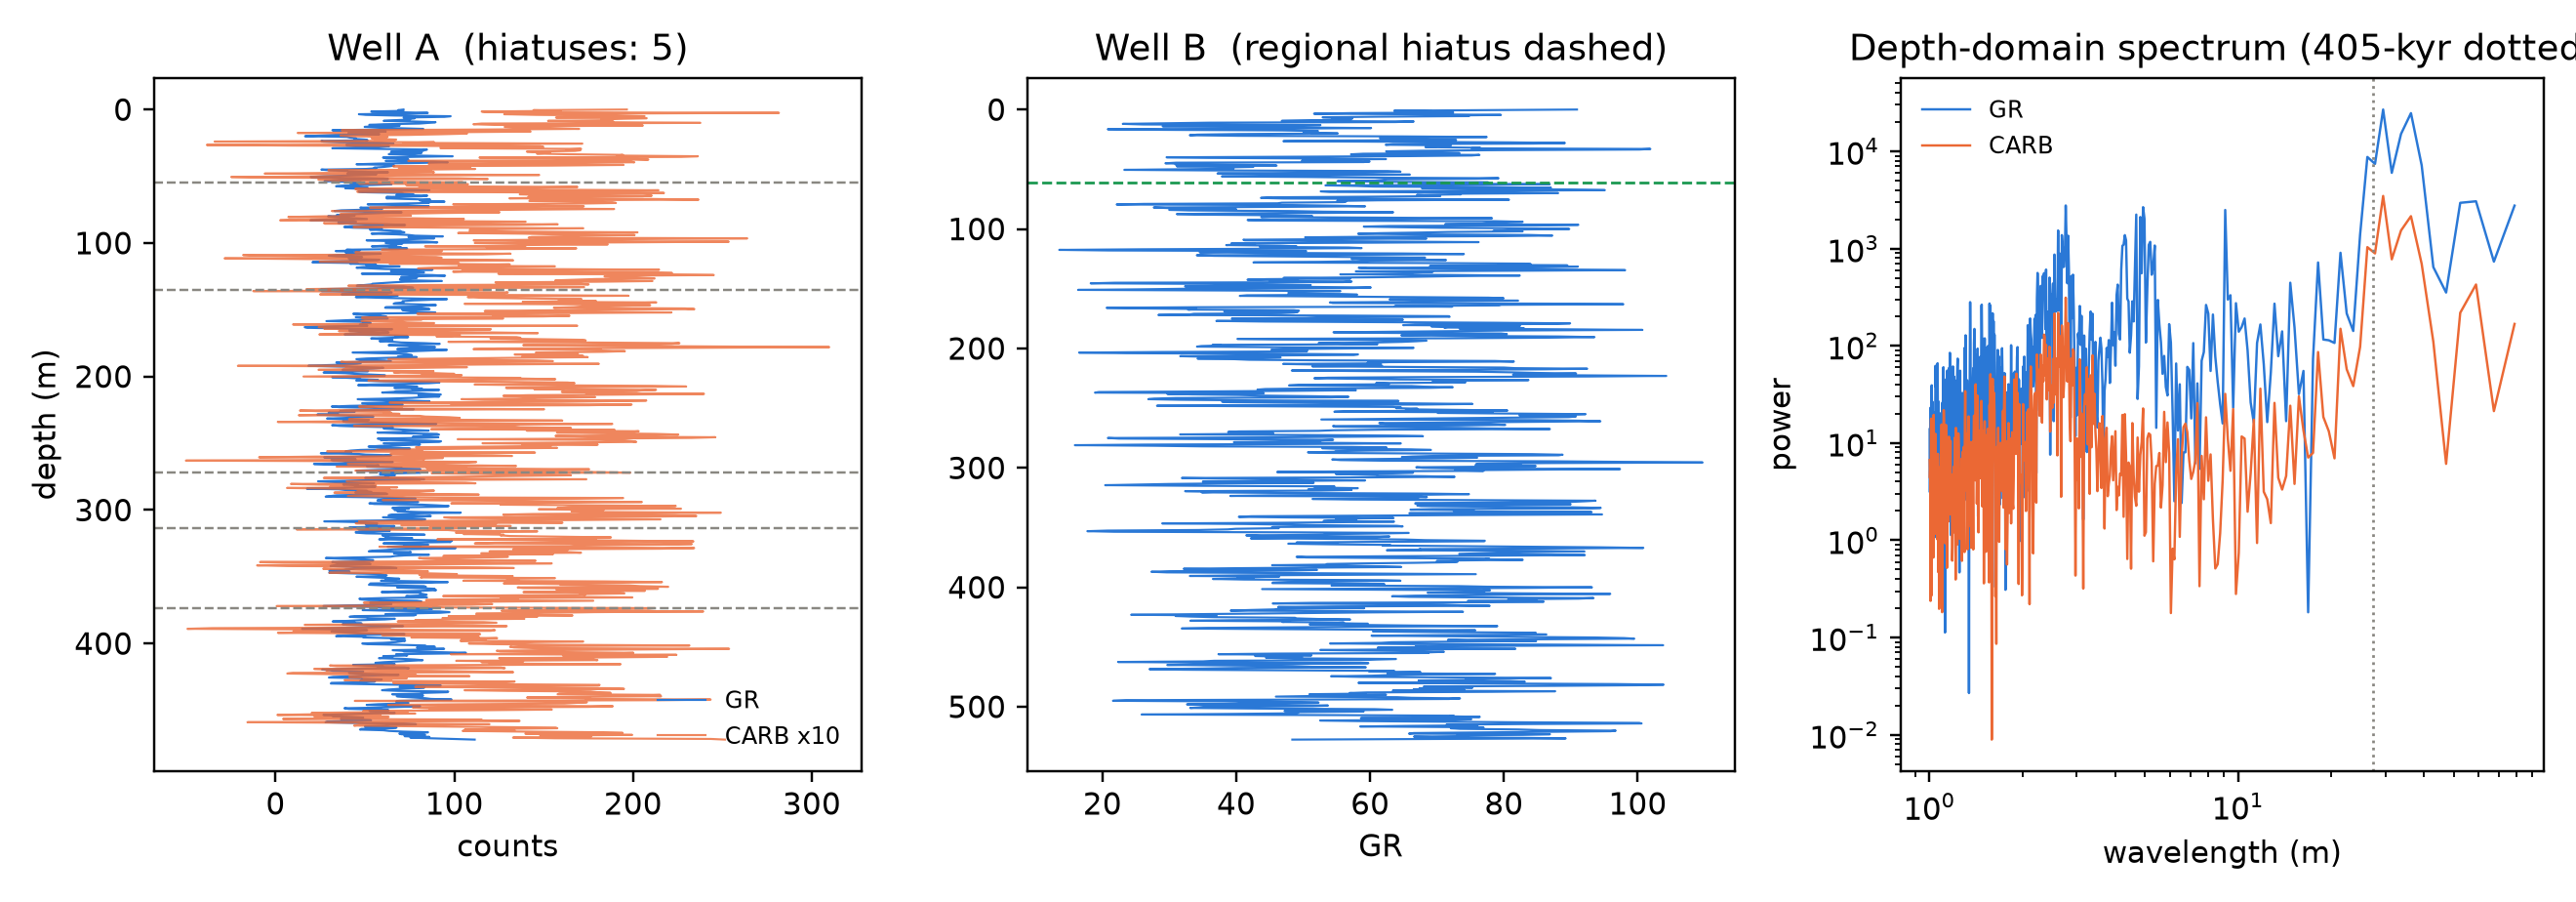
\includegraphics[width=\textwidth]{figures/fig1_instance.png}
\caption{A \method instance. Left: well A (GR and CARB) with the planted hiatus depths
(dashed). Middle: well B, where the shared regional hiatus sits at a different depth.
Right: depth-domain spectra; the dotted line marks the 405-kyr eccentricity wavelength
implied by the mean sedimentation rate.}
\label{fig:instance}
\end{figure}

\section{Experimental Setup}
\label{sec:setup}
% 1 page
\textbf{Models.} We evaluate five open chat models spanning one order of
magnitude in size: Qwen3-32B, DeepSeek-V3, GLM-4.6, Llama-3.1-70B, GPT-4o-mini, and a local
Qwen2.5-1.5B-Instruct that also serves as the GRPO base. Qwen3-32B and
Qwen3-14B were queried with hidden reasoning disabled (the vendor's enable\_thinking=False);
the other models ran with their default behaviour.

\textbf{Conditions.} Each instance is presented in one of three conditions. In
\emph{zero-shot} the model receives a data summary (size, depth range, sampling) and answers
from knowledge. In \emph{chain-of-thought} it is additionally asked to reason step by step.
In \emph{tool} the model receives the CSV paths and may execute Python (numpy/scipy/pandas)
in a sandbox for up to three turns before returning the JSON.

\textbf{Decoding and metrics.} We use temperature 0 and a 2048-token limit, with four
concurrent requests and three retries. The primary metric is the macro accuracy over the
eight questions; we also report per-family accuracy (Table~\ref{tab:main}) and, for the tool
condition, the fraction of instances where the executed code produced a finite result.

\textbf{Training.} The 40 training instances provide 320 question sets. GRPO uses a LoRA
adapter on Qwen2.5-1.5B-Instruct with eight generations per prompt and two rewards: the
fraction of correct answers (0--1) and a valid-JSON reward. We report benchmark accuracy on
the 20 held-out instances plus GSM8K accuracy before and after training as a retention check.

\textbf{Reproducibility.} The generator is deterministic given the instance id: re-running
it reproduces the truth file byte for byte. All result files are JSONL with the raw model
output, the parsed answer and the per-question score; the analysis and tolerance-sweep scripts
recompute every number in this section. API models were queried at temperature 0 with three
retries; the tool sandbox preloads numpy, pandas and scipy and blocks file, network and import
access.

\section{Results}
\label{sec:results}
% 1.5 pages
\subsection{Main results}
Table~\ref{tab:main} reports the macro accuracy over the 20 held-out instances (160 scored
questions per cell). No model comes close to solving the task: the best macro accuracy is
15.6\% (Qwen3.5-122B, zero-shot), and three of the five models stay below 3\%. A non-LLM
reference implementation of the textbook workflow, written for this paper, reaches 14.4\%
on the same instances -- the same range as the best model, which shows that the task is hard
for careful hand-written pipelines as well as for LLMs. Chain-of-thought prompting does not
help consistently (Qwen3.5-122B 15.6$\to$13.1, DeepSeek 10.0$\to$1.9, GLM-4.5-Air
1.9$\to$4.4), and the tool condition is no better than zero-shot (best 6.3\%). We return to
why in \S\ref{sec:analysis}. Bootstrap 95\% confidence intervals over instances overlap for
the top two models (Qwen3.5-122B 15.6 [11.9, 20.0], DeepSeek-V3.2 10.0 [6.9, 13.1]), so we do
not claim a ranking between them; the gap to the remaining models is larger than its interval.

\begin{table}[t]
\centering
\small
\begin{tabular}{@{}lccc@{}}
\toprule
Model & Zero-shot & CoT & Tool \\
\midrule
Qwen3.5-122B & 15.63 & 13.13 & 6.25 \\
DeepSeek-V3.2 & 10.00 & 1.88 & 5.00 \\
Qwen3-32B & 0.00 & 1.88 & 2.50 \\
GLM-4.5-Air & 1.88 & 4.38 & -- \\
Qwen3-14B & 2.50 & 1.25 & -- \\
\midrule
Reference solver (non-LLM) & 14.38 & -- & -- \\
\bottomrule
\end{tabular}
\caption{Macro accuracy (\%) over 20 held-out instances (160 scored questions per cell;
parse failures count as zero; --- marks a condition that did not complete). The reference solver is a Python implementation of the
textbook workflow, not the generator.}
\label{tab:main}
\end{table}
\begin{table}[t]
\centering
\small
\begin{tabular}{@{}lcccccccc@{}}
\toprule
Model (zero-shot) & Q1 & Q2 & Q3 & Q4 & Q5 & Q6 & Q7 & Q8 \\
\midrule
Qwen3.5-122B & 0 & 5 & 0 & 0 & \textbf{80} & 35 & 5 & 0 \\
DeepSeek-V3.2 & 0 & 0 & 0 & 0 & 35 & \textbf{45} & 0 & 0 \\
Qwen3-14B & 0 & 0 & 0 & 0 & 0 & 20 & 0 & 0 \\
GLM-4.5-Air & 0 & 0 & 0 & 0 & 0 & 10 & 5 & 0 \\
Qwen3-32B & 0 & 0 & 0 & 0 & 0 & 0 & 0 & 0 \\
\bottomrule
\end{tabular}
\caption{Per-question pass rate (\%) in the zero-shot condition. Q5 (the 300-Ma obliquity
period) is the only numeric question solved at scale; Q6 (orbital attribution) is partially
solvable; Q1--Q4 and Q8 are never solved.}
\label{tab:perq}
\end{table}

\begin{figure}[t]
\centering
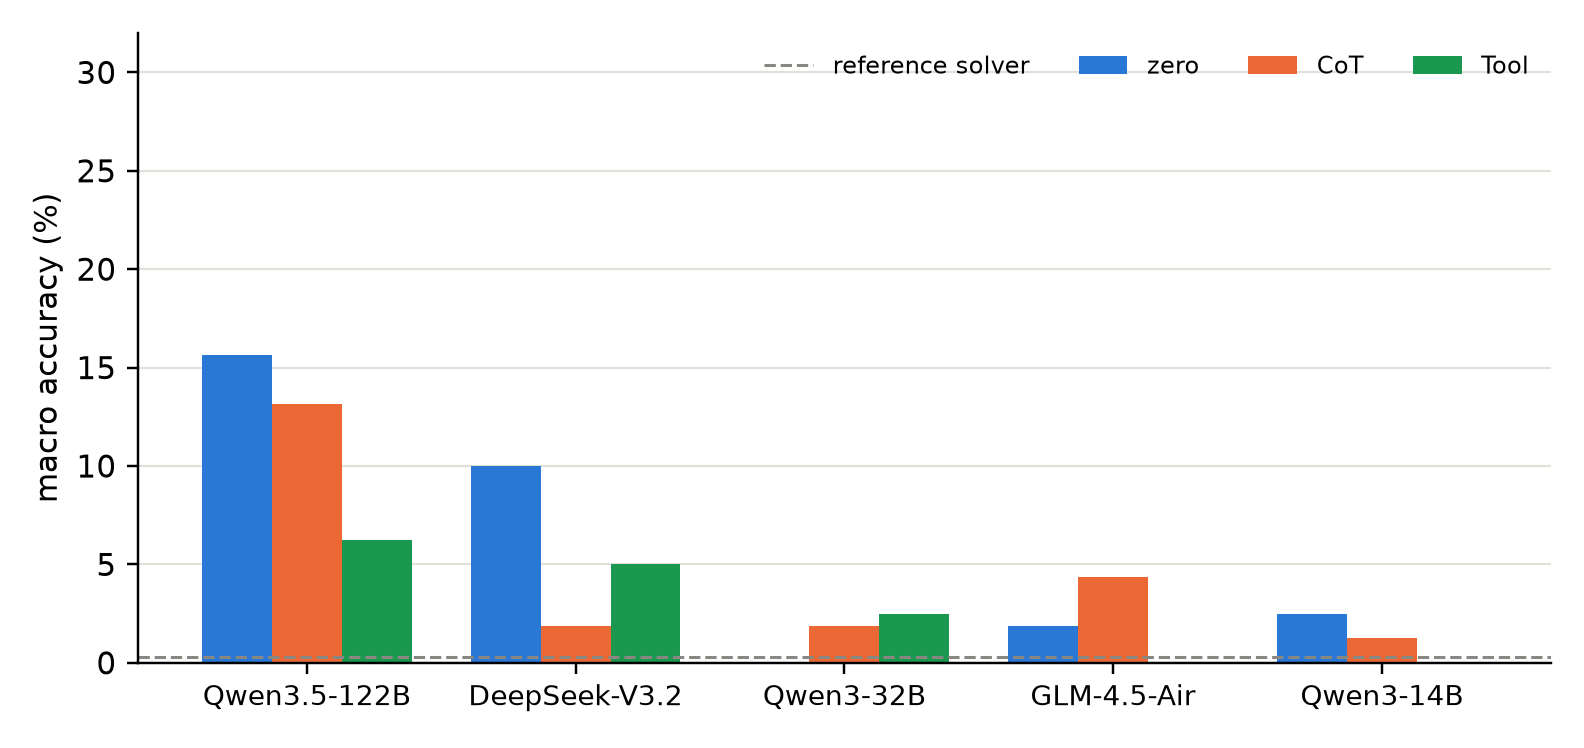
\includegraphics[width=0.92\textwidth]{figures/fig2_results.png}
\caption{Macro accuracy by model and condition (20 held-out instances). The dashed line is
the non-LLM reference solver; no model reaches half of it.}
\label{fig:results}
\end{figure}



\subsection{Error analysis}
\label{sec:analysis}
Across 260 model-instance runs, 94.6\% of the outputs parse as JSON, so parsing is not what
fails. The failures are numerical and structural. Q1--Q4 and Q8 almost never pass: models
report durations an order of magnitude too large (e.g., 97.7 Myr against a 7.0-Myr record) and
mean rates that are not on the right scale. Q5 (the 300-Ma obliquity period) is the only numeric question
solved at scale: Qwen3.5-122B passes 80\% of instances zero-shot, because the answer lies in a
narrow, well-known band. Q6 is partially solvable (DeepSeek 45\%), and Q7 is a binary direction
that is occasionally guessed. Q1--Q4 and Q8 are zero for every model. The 41-kyr shortcut is rare (6 of 246
parsed answers), because most models do not answer with a plausible period at all. On Q3,
83.3\% of answers report the wrong number of hiatuses, even when individual depths are within
a few metres; on Q6, 61.0\% get one to three of the four booleans right, i.e., partial
cross-validation rather than a coherent judgement. The tool condition does not fix this: the
models run code, but the outputs are not turned into a tuned age model (best macro 6.3\%).
The analysis script is public and recomputes all of these counts from a result file.

\begin{table}[t]
\centering
\small
\begin{tabular}{@{}llll@{}}
\toprule
Question & Truth & Model answer & Condition \\
\midrule
Q1 total duration & 5.27 Myr & 300.0 Myr & Qwen3-32B, tool \\
Q5 obliquity period & 32.4 kyr & 38.5 kyr & DeepSeek-V3.2, tool \\
Q3 hiatus count & 3 & 2 & DeepSeek-V3.2, CoT \\
\bottomrule
\end{tabular}
\caption{Representative errors. The first is a scale error of nearly two orders of magnitude;
the second is a plausible but out-of-band period; the third is a list-level mistake.}
\label{tab:errors}
\end{table}
To check whether the near-zero scores are an artefact of the tight tolerances, we re-scored
the same answers with every tolerance multiplied by 2, 5 and 10. The gain is steady but
small: Qwen3.5-122B rises from 15.6\% to 23.1\%, DeepSeek-V3.2 from 10.0\% to 25.0\%, and
Qwen3-32B from 0.0\% to 0.6\%. The answers are far from the truth, not merely outside a
narrow band.

\section{Future Work: Verifiable-Reward Post-Training}
\label{sec:grpo}
% 1.25 pages
\textbf{Recipe.} A natural use of \method\ is as a reward environment. We fine-tune Qwen2.5-1.5B-Instruct with a LoRA adapter (r=16, alpha=32,
all projection matrices) and train with GRPO on the 40 training instances (320 prompts).
Each prompt asks for the full JSON answer, so one completion receives a reward equal to the
fraction of its eight answers that the scorer accepts; a second reward gives partial credit
for a parseable JSON object. We use eight generations per prompt, a completion limit of 768
tokens, $\beta=0.04$, and a learning rate of $1\times10^{-6}$ for one epoch. Training runs on
a single A10 (23 GB) and is compared against the unadapted base on the 20 held-out instances.


\subsection{Status}
The recipe is released as code (\texttt{train\_grpo\_cyclobench.py}) with the same rewards and
splits. We deliberately do not report trained-model numbers in this version: the evaluation in
\S\ref{sec:results} is the baseline a training study must beat, and running it is the first item
of future work.

\section{Case Study: When the Tool Is Wrong}
\label{sec:case}
% 0.75 page
Tool-augmented evaluation assumes the tools are correct. In an earlier version of the benchmark
we found a Bayesian changepoint function in an open-source cyclostratigraphy package that
returned an all-zero posterior because the log-sum-exp was computed without the max-shift
trick; the underflow made every candidate changepoint equally unlikely. Models that called the
function and trusted it reported no hiatus, while models that inspected the posterior noticed
the degenerate output. The bug was fixed by a numerically stable implementation, and synthetic
tests then recovered all planted changepoints.

This episode motivates a design choice: the benchmark scores answers, not tool calls, so a model
can still succeed by checking tool output. It also suggests an adversarial variant in which one
tool is silently wrong; we leave that variant to future work and report only the correct-tool
setting here.

\section{Limitations and Conclusion}
\label{sec:conclusion}
% 0.25 page
Our benchmark is synthetic, single-domain, and English-only. The generator imposes a known
orbital model, so a model could in principle learn the generator's quirks rather than the
science; the held-out instances share the generator but not the parameters, and the truth is
computed from latent variables rather than from a solver, which limits circularity but does not
remove it. Model coverage is a snapshot of the current API landscape.

A second limitation is calibration. The tolerances were set from the generator's exact
parameters (e.g., 0.10 Myr on a 5--8 Myr record, 3 m on hiatus depth). A legitimate workflow
that estimates the sedimentation rate locally can miss these bands even when its analysis is
sound: our reference solver passes Q6 and Q7 almost always but never meets the numeric
tolerances on Q1--Q4. The current benchmark therefore measures exact recovery, not approximate
agreement, and part of the near-zero model scores reflects that choice. Two further
caveats: Q5 (the obliquity period) can be answered from prior knowledge of the 300-Ma
value, so a pass there is not evidence of data analysis; and the tool condition uses a
restricted sandbox with three turns and a truncated output, which may understate what a
better instrumented agent could do. Partial-credit
variants and tolerance sweeps are the obvious next step.

Within these limits, \method\ shows that verifiable scientific workflows can be measured with
exact answers, that current models score near zero without tools, and that a restricted sandbox
does not close the gap by itself. We release the generator, the 60 instances, the scoring code,
and the training recipe.

\bibliographystyle{plainnat}
\bibliography{refs}

\end{document}
